\documentclass[12pt]{article}
\setlength{\textwidth}{17cm}
\setlength{\textheight}{24cm}
\setlength{\topmargin}{-2cm}
\setlength{\footskip}{1cm}
\setlength{\evensidemargin}{0cm}
\setlength{\oddsidemargin}{0cm}
\setlength{\parindent}{0cm}

\usepackage{allrunes}
\usepackage{amsmath}
\usepackage[magyar]{babel}
\usepackage[T1]{fontenc}
\usepackage[utf8]{inputenc}
\usepackage{fixltx2e}
\usepackage{multirow}

\usepackage[hyphens]{url}
\usepackage[unicode,colorlinks=true,breaklinks]{hyperref}
%\usepackage[dvips]{hyperref}
%should display links, but it does not work with \H accent
%and formulas in section titles

\hypersetup{colorlinks,linkcolor=blue,urlcolor=magenta,citecolor=magenta}
%Breaks long url`s in text, while keeping it one link:

\usepackage{amsfonts}
\usepackage{amsthm}
\usepackage{amssymb}


\theoremstyle{plain}
\usepackage{graphicx}

%\usepackage{gensymb}
\usepackage{float}

% For bra-ket notation
\usepackage{braket}

%% New commands
\newcommand{\dd}{\textrm{d}}

%% Pauli matrices
\newcommand{\sigx}{\sigma_x}
\newcommand{\sigy}{\sigma_y}
\newcommand{\sigz}{\sigma_z}

\newcommand{\paulix}{
    \left( \begin{array}{cc}
        0 & 1 \\
        1 & 0
    \end{array}
    \right)
}

\newcommand{\pauliy}{
    \left( \begin{array}{cc}
        0 & -i \\
        i & 0
    \end{array}
    \right)
}

\newcommand{\pauliz}{
    \left( \begin{array}{cc}
        1 & 0 \\
        0 & -1
    \end{array}
    \right)
}


\begin{document}
\title{2. tétel}
\author{Nagy Dániel}
\maketitle


\newpage
\begin{abstract}
    Bootstrap módszerek. A maximum likelihood módszer. Hipotézis tesztelés. Extrém statisztikák.
    Post hoc analízis. Regresszió. Függetlenségvizsgálat. Egzakt tesztek.
\end{abstract}

\section{Bevezetés}
\subsection{Valószínűségszámítás alapfogalmak}
\begin{itemize}
    \item \textbf{Eseménytér} (ez egy abstrakt fogalom): $\Omega = \{\omega_1, \omega_2, ..., \omega_n\}$ pl. kockadobás esetén $\Omega = \{ \omega_1=\text{"1est dobok"}, \omega_2=\text{"2est dobok"}, \omega_3=\text{"párosat dobok"} ... \}$
    \item \textbf{Valószínűségi változó}: $X:\Omega \rightarrow \mathbb R$ pl. kockadobás esetén $X(\omega_1) = 1, X(\omega_2) = 2, ... $
    \item \textbf{Valószínűség}: $P$ egy mérték, amely $\Omega$ részhalmazaihoz számot rendel:
        \begin{itemize}
            \item $P: \mathcal{P}(\Omega) \rightarrow \mathbb R$
            \item $P(\Omega) = 1$ és $P(\varnothing) = 0$
            \item $ 0 \leq P(A) \leq 1 ~ \forall A \in \Omega$
            \item Ha $A_1, A_2, ...$ diszjunkt részhalmazai $\Omega$-nak, akkor 
            \begin{equation*}
                P\left(\bigcup\limits_{i=1}^{\infty}A_i\right) = \sum\limits_{i=1}^{\infty}P(A_i)
            \end{equation*}
        \end{itemize}
    \item \textbf{Hasznos összefüggések}:
        \begin{itemize}
            \item $P(A\cup B) = P(A)+P(B)-P(A\cap B)$
            \item Két esemény független $\Longleftrightarrow P(A\cap B) = P(A)P(B)$
            \item $P(A|B) = \frac{P(A\cap B)}{P(B)}$
            \item Teljes valószínűség: Ha $A_1, A_2, ...$ az $\Omega$ egy felosztása, akkor 
                \begin{equation*}
                    P(B) = \sum\limits_{k} P(B|A_k)P(A_k)
                \end{equation*}
            \item Bayes-tétel: Ha $A_1, A_2, ...$ az $\Omega$ egy felosztása, akkor 
                \begin{equation*}
                    P(A_k|B) = \frac{P(B|A_k)P(A_k)}{P(B)} = \frac{P(B|A_k)P(A_k)}{\sum\limits_{j} P(B|A_j)P(A_j)}
                \end{equation*}
        \end{itemize}
    \item \textbf{Eloszlásfüggvény} (CDF - cumulative distribution function):
        \begin{equation*}
            F_X(x) = P(X<x) = P(\{\omega\in\Omega | X(\omega)<x \})
        \end{equation*}
        diszkrét esetben 
        \begin{equation*}
            F_X(x) = P(X=x) = P(\{\omega\in\Omega | X(\omega)=x \})
        \end{equation*}
        Ha az $X$ változó $F$ eloszlást követ, akkor így jelöljük: $X\sim F$.
    \item \textbf{Sűrűségfüggvény} (PDF - Probability density function):\\
    Ha az $X$ változó eloszlásfüggvénye $F_X(x)$, akkor a sűrűségfüggvény definíciója
        \begin{equation*}
            F_X(x) = \int\limits_{-\infty}^{x}\rho_X(\xi)\dd \xi \Longleftrightarrow P(a \leq X(\omega) \leq b) = \int\limits_{a}^{b}\rho_X(x)\dd x
        \end{equation*}
        Megjegyzés: sűrűségfüggvénye csak folytonos eloszlású valószínűségi változónak van.
    \item \textbf{Várható érték}
    \begin{equation*}
        \text{folytonos eset}~E(X) = \langle X \rangle = \int\limits_{-\infty}^{\infty}x\rho(x) \dd x 
    \end{equation*}
    \begin{equation*}
        \text{diszkrét eset}~E(X) = \langle X \rangle = \sum\limits_{k} x_k p_k = \sum\limits_{k} x_k P(X=x_k)
    \end{equation*}
    \item \textbf{Várható értékre vonatkozó azonosságok}:
        \begin{itemize}
            \item Ha $Y=g(X) \Rightarrow E(Y) = E(g(X)) = {\displaystyle\int\limits_{-\infty}^{\infty}g(x)\rho(x) \dd x}$  
            \item ${\displaystyle E\left(\sum\limits_k a_k X_k\right) = \sum\limits_k a_k E(X_k)}$
            \item Ha $X_1, X_2, ...$ független változók, akkor ${\displaystyle E\left(\prod\limits_k X_k\right) = \prod\limits_k E(X_k)}$
        \end{itemize}
    \item \textbf{Variancia} (szórásnégyzet)\\
    Ha $E(X)=\mu$, akkor a szórásnégyzet a változó és a várható értéke közötti különbség négyzetének várható értéke:
    \begin{equation*}
        \sigma^2(X) = V(X) = E((X-\mu)^2) = \langle (X-\mu)^2 \rangle = \langle X^2 \rangle - \mu^2
    \end{equation*}
    \item Ha $X_1, X_2, ...$ függetlenek, akkor 
        \begin{equation*}
            \sigma^2\left( \sum\limits_k(a_kX_k + b_k) \right) = \sum\limits_k a_k^2\sigma^2(X_k)
        \end{equation*}
    \item \textbf{Szórás} (standard deviation) definíciója:
        \begin{equation*}
            \sigma(X) = \sqrt{\sigma^2(X)} = \sqrt{\langle X^2 \rangle - \langle X \rangle^2}
        \end{equation*}
    \item \textbf{Minta}\\
    Matematikailag egy statisztikai minta megfelel $N$ darab azonos eloszlású, független (iid) változónak egy adott $F$ eloszlásból.
    \item \textbf{Minta átlaga}: ${\displaystyle\overline{X} = \frac{1}{N}\sum\limits_{i=1}^{N}X_i}$ ($p_k$-t a relatív gyakorisággal közelítjük)
    \item \textbf{Minta varianciája}: ${\displaystyle s^2 = \frac{1}{N-1}\sum\limits_{i=1}^{N}(X_i-\overline{X})^2}$,
    standard hibája $SE = \sqrt{s^2}$. A nevezőben az $N-1$ faktor az ún. Bessel-korrekció \cite{besselcorr}.
    \item \textbf{Megjegyzés}: Ha egy teljes populáció esetén $E(X)=\mu$ és $V(X)=\sigma^2$, attól még általában
    $\overline{X}\neq\mu$ illetve $s^2\neq\sigma^2$.
    \item Egy minta esetében $\overline{X}, s^2, SE$ maguk is valószínűségi változók, hiszen minden mintavételezés esetén más-más
    értéket vehetnek fel. Ezért van értelme arról beszélni, hogy pl. $s^2$ értéke milyen eloszlást követ.
    Ha a minta (mérési pontok) iid változók, és $E(X_i)=\mu$, $V(X_i)=\sigma^2$, akkor 
    \begin{align*}
        & E(\overline{X}) = \mu \\
        & V(\overline{X}) = \sigma^2/N \\
        & E(s^2) = \sigma^2
    \end{align*}
\end{itemize}

\subsection{Statisztikai következtetés (inference)}
\begin{itemize}
    \item Az alapprobléma: van egy adathalmaz, ami tartalmazza a méréseket. Ezek $X_1, X_2, ..., X_N \sim F$ független, 
    azonos $F$ eloszlást követő valószínűségi változók.
    \item A statisztikai következtetés feladata, hogy a minta alapján meghatározzuk az $F$ eloszlásfüggvényt. Ezzel ekvivalens,
    ha $F$ helyett a $\rho$ sűrűségfüggvényt határozzuk meg.
    \item Ehhez használhatunk parametrikus és nem-parametrikus modelleket. A parametrikus modell egy olyan $\mathcal F$ halmaz, 
    ami a lehetséges PDF-eket tartalmazza:
    \begin{equation*}
        \mathcal F = \{\rho(x|\theta) : \theta \in \Theta\}\text{,}
    \end{equation*}
    ahol $\Theta$ a lehetséges paraméterek halmaza. Pl. ha normális eloszlást feltételezünk, akkor a parametrikus modell
    \begin{equation*}
        \mathcal F = \left\{\rho(x|\mu, \sigma) = \frac{1}{\sigma\sqrt{2\pi}}\exp\left(-\frac{(x-\mu)^2}{2\sigma^2}\right) : \mu\in\mathbb R, \sigma>0 \right\}\text{,}
    \end{equation*}
    a feladat pedig $\mu$ és $\sigma$ meghatározása. Nem-parametrikus modellek azok, amelyeket nem lehet véges számú valós paraméterrel
    definiálni, pl. $\mathcal F = \{\text{az összes létező PDF}\}$.
    \item \textbf{bias} Egy becsült $\hat\theta$ paraméter esetén a bias (előítélet, torzítás) alatt a becsült paraméter
    várható értéke és a valódi értéke közötti különbséget értjük \cite{biaswiki}: 
    \begin{equation*}
        Bias(\hat\theta) = E(\hat\theta) - \theta 
    \end{equation*}
\end{itemize}

\section{Bootstrap módszerek \cite{bootstrapwiki}}
A Bootstrap módszerek arra jók, hogy egy statisztikai minta esetén meghatározzuk a mérés pontosságát. 
A módszer lényege a következő: ahhoz, hogy az adott mérendő paraméter (pl. átlag) hibáját meg tudjuk mondani,
ismerni kellene a populáció adott paraméterét. Mivel ezt nem ismerjük, ezért a paraméter mérésének hibáját úgy
becsüljük, hogy a meglévő mintából sokszor újramintavételezünk, majd az újbóli mintavételezések alapján 
számítjuk ki a hibát. Ezzel az eljárással egy becslést kapunk az adott paraméter eloszlására.
Tehát a bootstrap módszer azzzal a feltételezéssel él, hogy a (minta $\rightarrow$ populáció) következtetés
egyenértékű az (újramintavételezés $\rightarrow$ minta) következtetéssel.
\par
\textit{Példa}. arra vagyunk kíváncsiak, hogy Magyarországon átlagosan milyen magasak az emberek. Mivel nem tudunk megmérni mindenkit,
ezért kiválasztunk $1000$ embert és lemérjük a magasságukat. Az átlagra a $\hat\mu$ értéket kapjuk. A kérdés az, hogy 
ez a $\hat\mu$ érték mennyiben tér el a valós $\mu$ értéktől? A választ úgy keressük, hogy az $1000$ adatból
véletlenszerűen újra mintavételezünk, így lesz sok $\hat\mu_i$ átlagunk és erre már kiszámíthatjuk a $V(\hat\mu)$ szórást.

\subsection{Jackknife módszer \cite{JackknifeWiki}}

A Jackknife egy olyan mintavételezési módszer, melynek segítségével különböző statisztikai paraméterek határozhatók
meg, mint pl. a variancia és a bias. 
A Jackknife módszer lényege, hogy az adott mintából mindig kihagyunk egy elemet, majd az így keletkező mintára újra 
kiszámoljuk az adott paramétert. Így kapunk egy eloszlást a becsült paraméterre, amelyből pontosabb eredményt kaphatunk.
\par
\textit{Példa}. A populáció átlagot akarjuk megbecsülni egy $n$ elemű mintából. Ehhez kiszámoljuk minden $n-1$ elemű
almintából az $\overline x_i$ átlagokat:
\begin{equation*}
    \overline x_i = \frac{1}{n-1}\sum\limits_{\substack{j=1 \\ j\neq i}}^{n} x_j
\end{equation*}
Ezután az átlag becslése az előbb kapott értékek átlaga:
\begin{equation*}
    \overline{x} = \frac{1}{n}\sum\limits_{i=1}^{n}\overline{x_i}
\end{equation*}
A Jackknife módszer alapján a becslés varianciája:
\begin{equation*}
    V(\overline{x}) = \frac{n-1}{n}\sum\limits_{i=1}^{n}(\overline{x}_i - \overline{x})^2
\end{equation*}


\section{Maximum likelihood}
A maximum likelihood módszer egy olyan becslési eljárás, amelynek segítségével egy parametrikus modell paramétereinek
értékét próbáljuk a minta alapján meghatározni. Ehhez felírjuk az ún. likelihood-függvényt, ami azt fejezi ki, hogy a 
mért adatok esetén mekkora a valószínűsége a $\theta$ paramétereknek. Ha a változó elposzlása ismert, akkor ezzel 
megadható a likelihood függvény:
\begin{align*}
    \text{diszkrét változóra:} ~ & \mathcal L(\theta) = P(X=x|\theta) \\
    \text{folytonos változóra:} ~ & \mathcal L(\theta) = \rho(x|\theta)
\end{align*}
A gyakorlatban sokszor a log-likelihood függvényt vagy az átlagolt log-likelihood függvényt használjuk:
\begin{align*}
    & \ell(\theta|x) = \ln \mathcal L(\theta|x) \\
    & \hat \ell(\theta|x) = \frac{1}{N}\ln \mathcal L(\theta|x)
\end{align*}
A maximum likelihood módszer lényege, hogy megkeressük azt a $\theta$ paramétert, ami a likelihood függvényt 
maximalizálja:
\begin{equation*}
    \hat\theta_{MLE} = \underset{\theta \in \Theta}{\textrm{argmax}} \,\mathcal L(\theta|x_1, x_2, ..., x_N)
\end{equation*}

\textbf{Példa:} normális eloszlás paraméterei\\
\begin{equation*}
    \rho(x|\mu, \sigma^2) = \frac{1}{\sigma\sqrt{2\pi}}\exp\left(-\frac{(x-\mu)^2}{2\sigma^2}\right)
\end{equation*}

Ezért egy $N$ elemű minta esetén azt feltételezve, hogy a mintát egy normális eloszlást követő populációból vesszük, 
az $N$ minta sűrűségfüggvénye:
\begin{align*}
  &  \rho(x_1, x_2, ..., x_N | \mu, \sigma^2) = \prod\limits_{i=1}^{N} \rho(x_i|\mu, \sigma^2)
    = \prod\limits_{i=1}^{N} \frac{1}{\sigma\sqrt{2\pi}}\exp\left(-\frac{(x_i-\mu)^2}{2\sigma^2}\right) \\
  & = \left(\frac{1}{2\pi\sigma^2}\right)^{n/2} \exp\left(-\frac{\sum\limits_{i=1}^N(x_i-\mu)^2}{2\sigma^2}\right)
    = \mathcal L(\mu, \sigma^2)
\end{align*}
A log-likelihood függvény pedig
\begin{equation*}
    \ell(\mu, \sigma^2) = \ln \mathcal L(\mu, \sigma^2) =
    -\frac{N}{2}\ln(2\pi\sigma^2) - \frac{1}{2\sigma^2}\sum\limits_{i=1}^{N}(x_i-\mu)^2
\end{equation*}
Ahhoz, hogy megkapjuk a $\hat\mu_{MLE}$ és $\hat\sigma_{MLE}$ becsült paramétereket, az alábbi két egyenletet kell megoldani:
\begin{align*}
    & \frac{\partial \ell(\mu, \sigma^2)}{\partial \mu} = 0 \\
    & \frac{\partial \ell(\mu, \sigma^2)}{\partial \sigma} = 0
\end{align*}
Ha ezeket megoldjuk, az jön ki, hogy $\hat\mu_{MLE} = \overline{x} = \frac{1}{N}\sum\limits_{i=1}^{N}x_i$ és 
$\hat\sigma_{MLE}^2 = \frac{1}{N}\sum\limits_{i=1}^{N}(x_i-\mu)^2$.

\section{Extrém statisztikák}
Az extrém statisztikák (extrémérték-elméletek) olyan események modellezésére alkalmazhatók, amelyek extrém ritkán fordulnak elő: pl. szökőár,
tőzsdei összeomlás, 100 éves hőmérsékleti rekord, stb. \cite{extremestat}.

Egy egyszerű egyváltozós modell a következő képpen írható le: Legyen $I_n$ annak a valószínűsége, hogy $n$ esemény során
bekövetkezik az extrém érték. Ezt úgy modellezzük, hogy veszünk $X_1, ..., X_n$ iid változót az $F$ eloszlásból.
Ekkor $M_n = \max(X_1, ..., X_n)$ esetén:
\begin{equation*}
    P(M_n < \leq z) = P(X_1\leq z, ..., X_n\leq z) = (F(z))^n
\end{equation*}
Az $I_n = I_n(M_n\geq z)$ így binomiális eloszlást követ, amelyre $p(z) = 1-(F(z))^n$. Az egy extrém esemény bekövetkezéséhez 
szükséges próbálkozások száma pedig geometriai eloszlást követ ugyanezzel a $p(z)$ paraméterrel.\cite{extremestat_univariate}

\section{Post-hoc analízis}
A post-hoc analízis azt jelenti, hogy csak azután választjuk ki a teszt statisztikát, miután már az adatokat ismerjük.
("post-hoc" = "ez után").
Ez a módszer többféle problémához vezethet, bővebben: \cite{posthoc, dredging}

\section{Regresszió}
Tegyük fel, hogy a megfigyelt adathalmaz $\{(x_1, y_1), (x_2, y_2), ..., (x_N, y_N)\}$. Ekkor az $X$ a független változó
(feature variable, predictor, regressor), $Y$ pedig a függő változó (outcome, response variable).
Az \textbf{\textit{$r(X)$ regressziós függvény}} az $Y$ várható értéke $X$ függvényében:
\begin{equation*}
    r(x) = E(Y|X=x)
\end{equation*}
\begin{itemize}
    \item Ha $r(x)$ megadható véges számú valós paraméterrel, akkor \textbf{parametrikus regresszió}ról beszélünk.
    \item Ha $Y$ meghatárzása a cél, ismert $X$ esetén, akkor \textbf{predikció}ról beszzélünk.
    \item Ha $Y$ diszkrét (pl. kutya vagy macska látható a képen), akkor \textbf{klasszifikáció}ról beszélünk.
    \item Ha a cél az $r(x)$ görbe meghatározása, akkor \textbf{regresszió}ról vagy \textbf{görbeillesztés}ről beszélünk.
\end{itemize}

\section{Hipotézistesztelés}
A hipotézistesztelés lényege, hogy a rendelkezésre álló adatok alapján egy feltevés (hipotézis) igazságtartalmára akarunk
kijelentést tenni. Fontos, hogy a feltevés a teljes populációra vonatkozik, tehát egy hipotézis elfogadásának vagy elutasításának
mindig van valamennyi bizonytalansága. Példák: 1. Dobunk egy dobókockával 100-szor, majd feltesszük azt a hipotézist, hogy 
a dobott számok egyenletes eloszlást követnek. 2. Megnézzük 1000 ember jövedelmét majd feltételezzük, hogy a jövedelem olyan
lognormális eloszlást követ, amelyre $\mu=150000\text{HUF}$ és $\sigma=50000\text{HUF}$.
\par Formális definíció:
\begin{itemize}
    \item A $\Theta$ paraméter-teret felosztjuk $\Theta_0$ és $\Theta_1$-re. ($\Theta_0\cup\Theta_1=\Theta,\, \Theta_0\cap\Theta_1=\varnothing$)
    \item A \textbf{nullhipotézis}  $H_0:\, \theta\in\Theta_0$
    \item Az \textbf{alternatív hipotézis}  $H_1:\, \theta\in\Theta_1$
    \item Az összegyűjtött $X\in\mathcal X$ adatok alapján akarjuk a hipotézist eldönteni.
    \item Az elvetési régió (rejection region) egy $R\subset \mathcal X$ halmaz, amelyre
        \begin{align*}
            & X\in R \Rightarrow \text{$H_0$-t elvetjük és elfogadjuk $H_1$-et} \\
            & X\notin R \Rightarrow \text{$H_0$-t elfogadjuk}
        \end{align*}
    \item Egy tesztfüggvény (test statistic) egy $T: \mathcal X \rightarrow \mathbb R$ függvény, amelyre az elvetési
    régió így írható: 
        \begin{equation*}
            R = \{x \in \mathcal X | T(x) > c \} \text{, }
        \end{equation*}
    ahol $c$ a teszt kritikus értéke.
    \item A hipotézis tesztelés lényege keresni egy olyan $T$-t és $c$-t, amivel a legjobb (legkevésbé káros) döntést
    hozhatjuk.
    \item \textbf{Egyoldalú teszt}: Ha $X$ a rendelkezésre álló adathalmaz, és $\theta\in \Theta$ egy paraméter 
    (pl. átlag, variancia, stb), akkor egy egyoldalú teszt a következőt jelenti:
    \begin{equation*}
        H_0: \theta = \theta_0 ~\text{és}~ H_1: \theta < \theta_0 ~ (\text{vagy} > \theta_0) 
    \end{equation*}
    \item \textbf{Kettős hipotézisteszt}: Ha $X$ a rendelkezésre álló adathalmaz, és $\theta\in \Theta$ egy paraméter 
    (pl. átlag, variancia, stb), akkor egy kettős teszt a következőt jelenti:
    \begin{equation*}
        H_0: \theta = \theta_0 ~\text{és}~ H_1: \theta \neq\theta_0 
    \end{equation*}
    \item \textbf{Hibák}
    \begin{center}
        \begin{tabular}[H]{|c|c|c|} \hline
                            &        $H_0$ igaz        & $H_0$ hamis \\ \hline
        Elfogadjuk $H_0$-t  &      OK   &   type 2 hiba (false positive)  \\ \hline
        Elvetjük $H_0$-t    & type 1 hiba (false negative)  &      OK     \\ \hline
        \end{tabular}
    \end{center}
    \begin{figure}[H]
        \begin{center}
        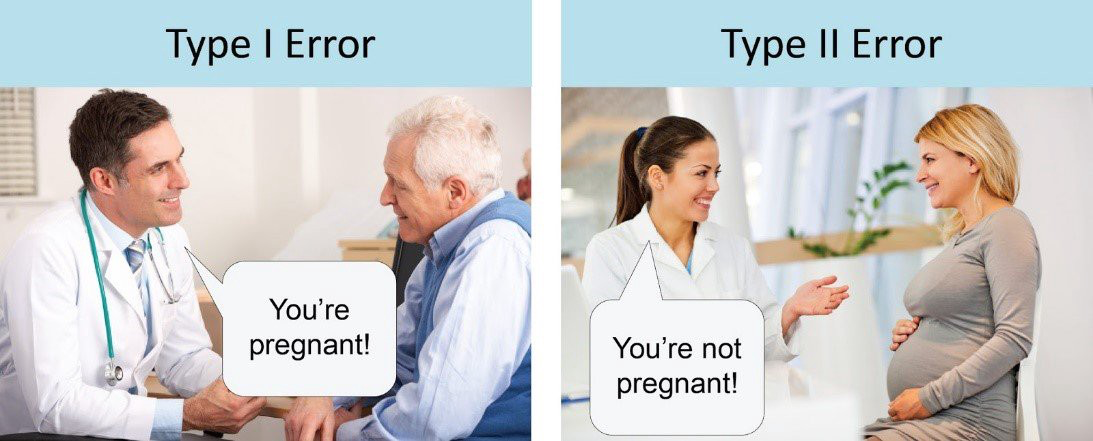
\includegraphics[width=0.75\textwidth]{media/typeoferrs.png}
        \caption{A két hibatípus.} 
        \label{fig:typeoferrs}
        \end{center}
    \end{figure}
    \item \textbf{Statisztikai erő}: Egy kettős hipotézisteszt statisztikai ereje nem más, mint az a valószínűség,
    hogy a teszt helyesen veti el a nullhipotézist, amikor az alternatív hipotézis igaz:
    \begin{equation*}
        \text{statisztikai erő} = \beta = P(H_0 \,\text{elutasítva} \,|\, H_1 \,\text{igaz})
    \end{equation*}
    \item \textbf{szignifikancia-szint} Egy statisztikai teszt $\alpha$ szignifikancia szintű, ha 
    a nullhipotézis elvetésének a valószínűsége $\alpha$ feltéve, hogy a nullhipotézis igaz.
    \begin{equation*}
        \alpha = P(\text{$H_0$-t elvetjük}\,|\,\text{$H_0$ igaz})
    \end{equation*}
    \item \textbf{p-érték}: A p-érték azt mutatja meg, hogy ha igaz a nullhipotézis, akkor mekkora 
    valószínűséggel kapunk olyan eredményt, amely legalább annyira extrém, mint a mért eredmény.
    Pl. Ha egy minta átlaga $\overline{X}$, akkor a $p=5\%$ azt jelenti, hogy ha a populáció átlaga $\mu$,
    akkor $5\%$ valószínűséggel mérhetek legalább $|\overline{X}-\mu|$ eltérést. A $p$-értéket így is definiálhatjuk:
    \begin{equation*}
        p = P(\text{ezt az eredményt mérem}\,|\,\text{$H_0$ igaz})
    \end{equation*}
    
\end{itemize}
\subsection{Egymintás $u$-próba \cite{uprobawiki}}(angolul z-test \cite{ztestwiki})
\begin{itemize}
    \item Egymintás $u$-próbával a minta alapján a populáció átlagára vonatkozó hipotézist lehet tesztelni.
    \item A populációt normális eloszlásúnak feltételezzük, melynek ismerjük a $\sigma$ szórását.
    \item Ha a $\sigma$ szórás nem ismert, akkor a $u$-próba helyett $t$-próbát kell végezni.
    \item Azt akarjuk megvizsgálni, hogy a minta alapján a $\mu$ érték tekinthető-e a populáció átlagának.
    \item A teszt elvégzéséhez kiszámoljuk a minta $\overline{X}$ átlagát, majd ebből a próbastatisztikát:
        \begin{equation*}
            u = \frac{\overline{X}-\mu}{\sigma/\sqrt{n}}
        \end{equation*}
    \item Kihasználjuk azt a feltételt, hogy az $u$ próbastatisztika standard normális eloszlást követ, és adott előre
    meghatározott $p$-értékre kiszámoljuk a $u_{p/2} = \Phi^{-1}(1-p/2)$-t. 
    \item Ha $|u| \geq u_{p/2}$, akkor ez azt jelenti, hogy a mért $\overline{X}$ és a feltételezett $\mu$ érték között
    $p$ szignifikancia-szint mellett az eltérés szignifikáns. Tehát elvetjük a nullhipotézist, miszerint a populáció átlaga $\mu$.

    \item \textbf{Példa:} Begyűjtünk 3 tonna almát, amiről tudjuk, hogy az almák tömegének szórása $\sigma=40g$.
    Találomra kiválasztunk 100db almát, amelyeket megmérve azt kapjuk, hogy a tömegek átlaga $\overline{X}=150g$.
    Kijelenthető-e $95\%$-os biztonsággal, hogy a begyűjtött almák átlagos tömege $\mu=140g$? És $99\%$-os 
    biztonsággal?
    \begin{itemize}
        \item $H_0: \mu = 140g$
        \item $H_1: \mu \neq 140g$
        \item $p_1=0.05,\,p_2=0.01$
        \item $u_{p_1/2} = \Phi^{-1}(1-p_1/2) = \Phi^{-1}(1-0.05/2) \approx 1.96$
        \item $u_{p_2/2} = \Phi^{-1}(1-p_2/2) = \Phi^{-1}(1-0.01/2) \approx 2.58$
        \item $u = {\displaystyle\frac{\overline{X}-\mu}{\sigma/\sqrt{n}}} = {\displaystyle \frac{150-140}{40/10}} = 2.5$
        \item WTF???
    \end{itemize}
\end{itemize}

\subsection{Egymintás $t$-próba \cite{tprobawiki}}
\begin{itemize}
    \item A vizsgált valószínűségi változó normális eloszlást követ, de nem ismerjük a $\sigma$ szórást.
    \item A kérdés ugyanaz, mint az előbb, hogy a populáció átlaga megegyezik-e statisztikai szempontból a
    feltételezett $\mu$ értékkel.
    \item $t$-próba esetén a próbastatisztika a következő lesz:
        \begin{equation*}
            t = \frac{\overline{X}-\mu}{s/n} \,\text{,}
        \end{equation*}
        ahol ${\displaystyle s = \sqrt{\frac{1}{n-1}\sum\limits_{i=1}^{n}(X_i-\overline{X})^2}}$ a minta szórása. A próbastatisztika
        ebben az esetben Student t-eloszlást követ, $f=n-1$ szabadsági fokkal.
    \item Az előbbihez hasonlóan az adott $p$ szignifikancia szinthez megkeressük a $t_p$ értéket.
    \item Ha $|t| \geq t_p$, akkor a nullhipotézist elvetjük, mert a minta átlaga szignifikánsan eltér a $\mu$ értéktől.
    \item Ellenkező esetben, vagyis ha $|t| < t_p$, a nullhipotézist megtartjuk.
\end{itemize}

\section{Függetlenségvizsgálat, $\chi^2$-próba}
A függetlenségvizsgálat arra szolgál, hogy eldöntsük, két diszkrét változó között, adott konfidenciaszinten van-e
összefüggés, vagy ez csupán a véletlen mintavételezés következménye. A változók lehetnek nominálisak (pl. fizetés)
vagy kategoriálisak (pl. nem). Folytonos változók (pl. életkor, fizetés, magasság) esetén ezeket diszkrétté tesszük, 
úgy hogy felosztjuk véges számú intervallumra. Ahhoz, hogy megállapítsuk, a mért gyakoriságok szignifikánsan eltérnek-e
a véletlen mértékétől, ún. Pearson-féle $\chi^2$-próbát kell végezni. Ennek a menete a következő:
\begin{itemize}
    \item első lépésben kiszámoljuk a teszt statisztikát: $\displaystyle{\chi^2 = \sum\limits_{i=1}^{n} \frac{(O_i-E_i)^2}{E_i}}$, ahol
    \begin{itemize}
        \item $O_i$ a mért értékek
        \item $E_i$ a várt elméleti értékek
        \item $\chi^2$ a teszt-statisztika, ami aszimptotikusan a $\chi^2$ eloszláshoz tart
    \end{itemize}
    \item Megállapítjuk a szabadsági fokok számát. Függetlenségvizsgálat esetén ez $df=(R-1)(C-1)$, ahol
    $R$ az egyik $C$ pedig a másik változó kategoriáinak száma (pl. ha azt vizsgáljuk, hogy van-e összefüggés a nemek és 
    a magasság között, akkor $R=2$ és $C=10$, ha a magasságot $10$ csoportra osztjuk).
    \item Meghatározunk egy szignifikancia szintet pl $95\%$.
    \item Összehasonlítjuk a kiszámolt $\chi^2$ értéket kritikus $\chi^2_t$ értékkel. $\chi^2_t$ függ a választott
    szignifikancia szinttől és a szabadsági fokok számától.
    \item A két érték összehasonlításával elfogadjuk, vagy elvetjuk a nullhipotézist (a nullhipotézis általában az, hogy
    a két változó között adott szignifikancia szinten van összefüggés.)
\end{itemize}
Konkrét számolásos példákat ebben a jegyzetben lehet találni: \cite{chi2jegyz}



\bibliographystyle{plain} 
\bibliography{references}

\end{document}
